\documentclass{article}
\usepackage{fullpage,amsmath,amsthm,graphicx,enumitem,amssymb}
\usepackage[hidelinks]{hyperref}
\usepackage{todonotes}
\theoremstyle{definition}
\newtheorem{thm}{Theorem}
\newtheorem{question}[thm]{Question}
\newenvironment{solution}{\noindent\textit{Solution:}}{}

\newcommand{\reals}{\mathbb{R}}

\title{ASEN 5519-003 Decision Making under Uncertainty\\
       Homework 2: Markov Decision Processes}

\begin{document}

\maketitle

\section{Conceptual Questions}

\begin{question} (10 pts)
    Give an example of an MDP with a unique nonzero optimal value function, but multiple optimal policies.\footnote{Hint: you can do this with $|\mathcal{S}| = 1$.}
\end{question}

\begin{question} (20 pts)
    Consider a stationary infinite-horizon MDP with $\mathcal{S} = \{1,2\}$, $\mathcal{R}(s, a) = s^2$, and $\gamma = 0.9$ ($\mathcal{A}$ and $\mathcal{T}$ are unknown). Suppose that policy $\pi$ achieves a value at state $1$ of $V^\pi(1) = 37$. What is $V^*(2)$, the optimal value at state $2$? Justify your answer.
\end{question}

\begin{question} (20 pts)
    Consider a 1 by 9 grid world with a key in cell 2 and a locked door in cell 8. An agent automatically receives a reward of 10 upon returning to cell 8 after having collected the key, and the problem terminates immediately. At each time step, the agent can take one of two actions, \texttt{left}, or \texttt{right} which always succeeds in moving the desired direction. If an end wall is hit, the agent bounces back to the previous cell. The discount factor is $\gamma=0.95$.
\begin{center}
    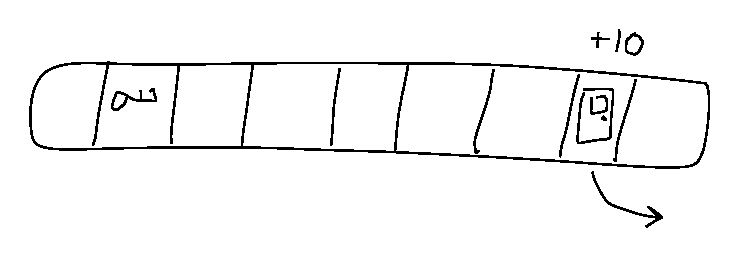
\includegraphics[width=0.5\textwidth]{small_mdp.pdf}
\end{center}

\begin{enumerate}[label=\alph*]
        \item Formulate this problem as an MDP, and write down the state space $\mathcal{S}$, reward function $\mathcal{R}$, and transition distributions $\mathcal{T}$.
        \item What is the value of being in cell 9 without the key?
    \end{enumerate}

\end{question}

\section{Exercise}

\begin{question} \label{q:gw}
    (Value iteration for Grid World, 25 pts)

    Solve the MDP \texttt{HW2.grid\_world} with your own implementation of value iteration with a discount of $\gamma=0.95$ and plot the resulting value function. All of the necessary information to solve this problem can be extracted with the \texttt{HW2.transition\_matrices} and \texttt{HW2.reward\_vectors} functions, and plotting can be accomplished with \texttt{HW2.render(HW2.grid\_world, v)} where \texttt{v} is the value function. See the starter code and function docstrings for more information.
\end{question}

\section{Challenge Problem}

\begin{question}
    (Value iteration for ACAS, 25 pts)

Your task is to find the optimal value function for an Aircraft Collision Avoidance System (ACAS). The encounter model will be specified as a Markov decision process, and your task will be to compute the value function for discount $\gamma=0.99$ using value iteration or another suitable algorithm that you implement. The continuous physical state space will be discretized at various levels of granularity and the goal is to find the value function for the finest discretization possible.

A model with discretization level \texttt{n} can be constructed with
\begin{verbatim}
                        m = HW2.UnresponsiveACASMDP(n)
\end{verbatim}
The higher \texttt{n} is, the finer the discretization and the larger the state space. Again, all of the information needed to solve this problem can be extracted with the \texttt{HW2.transition\_matrices} and \texttt{HW2.reward\_vectors} functions, so you can start with your code from Question \ref{q:gw}.

The score received for solving the problem is \texttt{n}. You must submit your code for this problem along with the \texttt{results.json} file from executing \texttt{HW2.evaluate(v, "email@colorado.edu")} where \texttt{v} is the value function vector. A score of \texttt{n} = 7 or higher will receive full credit\footnote{By taking advantage of the structure of the problem, it is possible to attain a score of \texttt{n} = 20 with less than 10 minutes of computation time on a single core of a i7 laptop processor.}.

\vspace{1em}
\noindent\makebox[\linewidth]{\rule{\textwidth}{0.4pt}}
\vspace{1em}

\textbf{The information above this line is sufficient to complete this homework.} However, the description of the model below may help to get the highest score on the leaderboard. The \texttt{UnresponsiveACASMDP} model implements the POMDPs.jl explicit MDP interface\footnote{\url{https://juliapomdp.github.io/POMDPs.jl/stable/dynamics/\#Separate-explicit-or-generative-definition}}, and students are welcome to explore the problem further using that interface as well as ask on Piazza and look at the source code for details. The underlying continuous model is defined as follows:

\begin{center}
    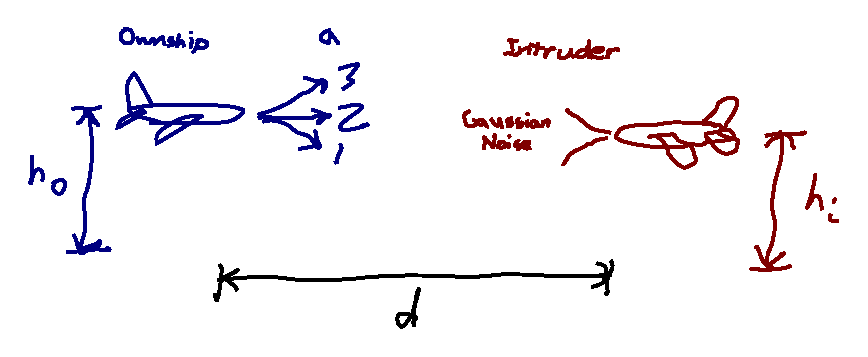
\includegraphics[width=0.7\textwidth]{unresponsive_acas.pdf}
\end{center}

\begin{itemize}
    \item The state space is 4-dimensional $\mathcal{S} = \reals^4$, with each state consisting of $s=(h_o, \dot{h}_o, h_i, d)$ where $h_o$ is the ownship altitude in feet, $\dot{h}_o$ is the rate of climb in ft/min, $h_i$ is the intruder altitude in feet, and $d$ is the distance between the aircraft in feet.
    \item The action space is $\mathcal{A}=\{-1500, 0, 1500\}$ and represents the change in rate of climb. The possible rates of climb are $\dot{h}_o \in \{-3000, -1500, 0, 1500, 3000\}$
    \item A reward of -100 is received for a near-mid-air collision, defined as the aircraft passing within 500 vertical feet and 100 horizontal feet of each other. Any change in rate of climb yields a reward of -1.
    \item The rate of climb, $\dot{h}_o$ changes instantly when an action is applied. Then the following dynamics are used: $d' = d - 2\,v\,\Delta t$ where $v$ is the fixed horizontal velocity, $h_o' = h_o + \dot{h}_o\,\Delta t$, and $h_i' = h_i + W_{\Delta t \sigma^2}$ where $W$ is the Wiener process\footnote{\url{https://en.wikipedia.org/wiki/Wiener_process}}. $\Delta t$ changes based on the discretization \texttt{n}.
\end{itemize}


\end{question}

\end{document}
